%Template file for MATH96012 project 2 discussion and figures
\documentclass{article}
\usepackage[utf8]{inputenc}
\title{MATH96012 Project 2}

\author{\emph{Alexander John Pinches CID:01201653}}

\usepackage{graphicx}

\begin{document}

\maketitle

%---------------- Question 1.3 -------------------

\section*{Part 1.3}
I chose the second version of the cost function as this allowed for vectorisation making it faster the principle disadvantage being this is only applicable in the CLR case.

%---------------- End Question 1.3 -------------------

%---------------- Question 2.3 -------------------

\section*{Part 2.3}
In python the code would be much more readable and easier to debug without the difficulties inherent in compiled languages and in python sticking to numpy esentially means running blocks of compiled C so is very fast. 
However Fortran will be faster because of optimisations made by the compiler across the whole algorithm and as we are evaluating this function many times small speed ups in individual runs can make a large difference to the overall time.

%---------------- End Question 2.3 -------------------


%---------------- Question 2.4 -------------------

\section*{Part 2.4}
In figure \ref{fig21} we see that MLR achieves close to if we classified at random error rates for all m where as neural networks achieve close to 0 error rate. The only disadvantage of the neural networks is the increased training time for small m. This shows for this problem that neural betworks are far superior. The two series are seperated out with LR in figure \ref{lr} and the NN in figure \ref{nn}. We see a clear increase in error rate as the number of classes for mlr however for nn we see the error rate remaining seemingly constant at 0. Highlighting how much better the predictive ability of the NN is. 
\subsection*{Figures}
\begin{figure}[h!]
\centering
%Uncomment line below to display figure saved as fig21.png
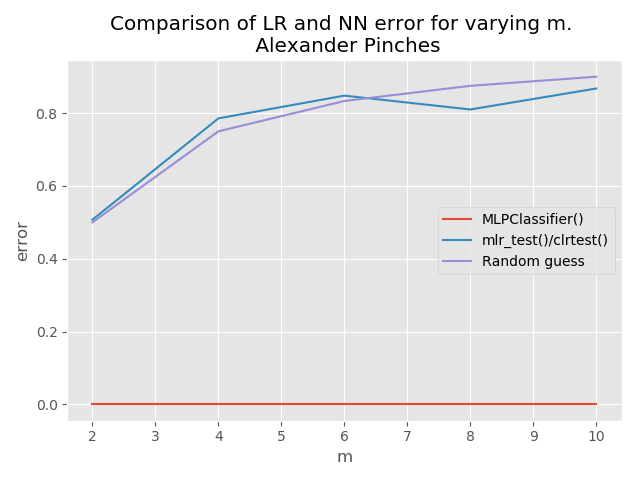
\includegraphics[width=0.6\textwidth]{graph.png}
\caption{Figure for question 2.4 showing the error over m for mlr and neural networks}
\label{fig21}
\end{figure}
\begin{figure}[h!]
\centering
%Uncomment line below to display figure saved as fig21.png
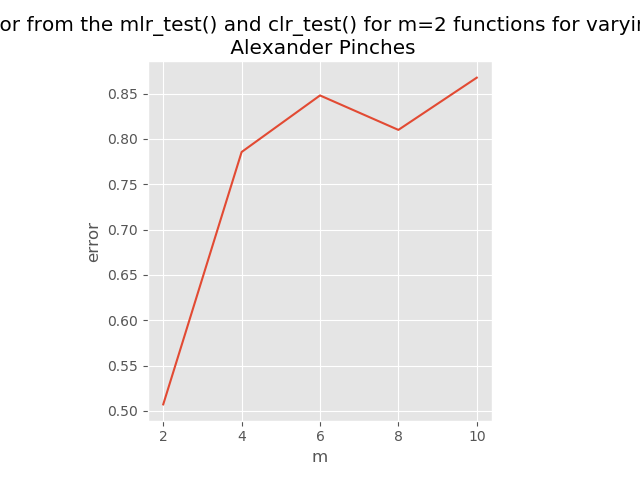
\includegraphics[width=0.6\textwidth]{graphLR.png}
\caption{Figure for question 2.4 showing the error over m for mlr}
\label{lr}
\end{figure}
\begin{figure}[h!]
\centering
%Uncomment line below to display figure saved as fig21.png
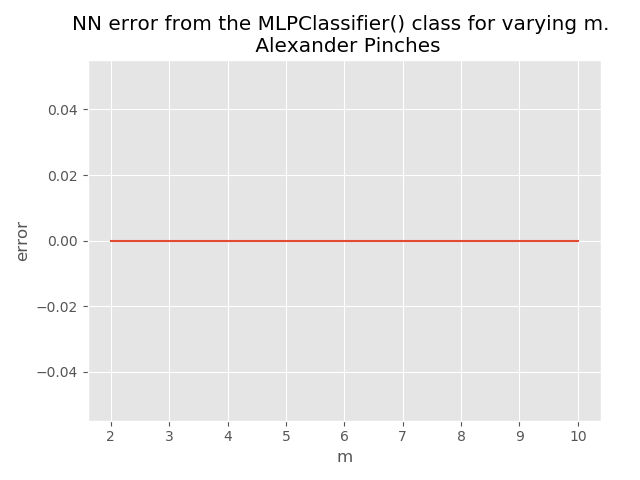
\includegraphics[width=0.6\textwidth]{graphNN.png}
\caption{Figure for question 2.4 showing the error over m for neural networks}
\label{nn}
\end{figure}

%Add further figures as needed here

%---------------- End Question 2.4 -------------------





%---------------- End document -------------------


\end{document}
